\documentclass{beamer}
\usepackage{mathrsfs,xcolor,setspace,comment,centernot,listings,framed,subfig,ragged2e}
\usepackage[utf8]{inputenc}
\usepackage[T1]{fontenc}

\DeclareMathOperator{\Cov}{Cov}
\DeclareMathOperator{\Var}{Var}
\DeclareMathOperator{\E}{\mathbb{E}}
\DeclareMathOperator{\Proba}{\mathbb{P}}

\newcommand{\Covb}[2]{\ensuremath{\Cov\!\left[#1,#2\right]}}
\newcommand{\Eb}[1]{\ensuremath{\E\!\left[#1\right]}}
\newcommand{\Pb}[1]{\ensuremath{\Proba\!\left[#1\right]}}
\newcommand{\Varb}[1]{\ensuremath{\Var\!\left[#1\right]}}

% norm
\newcommand{\norm}[1]{\| #1 \|}

\newcommand{\indep}{\rotatebox[origin=c]{90}{$\models$}}



% config du theme metropolis
\usetheme[progressbar=frametitle,block=fill, titleformat=smallcaps,sectionpage=progressbar,]{metropolis}



\title{Classifying Knowledge Domains of Theoretical and Quantitative Geography publications}
\subtitle{}

\date{06/02/2026\\
\textbf{TheoQuant 2026}\\
Session: \textit{Quelle place pour une géographie théorique}\\
et quantitative critique ?}

\author{Juste Raimbault\textsuperscript{1,2,3,4}}
\institute{\textsuperscript{1}LaSTIG, IGN-ENSG-UGE\\
\textsuperscript{2}CASA, UCL\\
\textsuperscript{3}UPS CNRS 3611 ISC-PIF\\
\textsuperscript{4}UMR CNRS 8504 Géographie-cités
}



%definition de la couleur du texte dans la balise \alert{}
\definecolor{vertIGN}{HTML}{96C31E} % vert IGN %vrai valeur #97BE0D
\setbeamercolor{alerted text}{fg=vertIGN}

\definecolor{grisIGN}{HTML}{22292F} % Gris IGN tiré vers le noir 
\setbeamercolor{background canvas}{bg=grisIGN}


% code pour placer le log ENSG dans le bandeau de titre 
\makeatletter
\setbeamertemplate{frametitle}{%
  \nointerlineskip%
  \begin{beamercolorbox}[%
      wd=\paperwidth,%
      sep=0pt,%
      leftskip=\metropolis@frametitle@padding,%
      rightskip=\metropolis@frametitle@padding,%
    ]{frametitle}%
  \metropolis@frametitlestrut@start%
  \insertframetitle%
  \nolinebreak%
  \metropolis@frametitlestrut@end%
  \hfill
  \raisebox{-0.6ex}{
\includegraphics[height=4ex,keepaspectratio]{figures/logoENSG_small.jpg}}
  \end{beamercolorbox}%
}


\newcommand{\noun}[1]{\textsc{#1}}
\newcommand{\jitem}[1]{\item \begin{justify} #1 \end{justify} \vfill{}}
\newcommand{\sframe}[2]{\frame{\frametitle{#1} #2}}

\newenvironment{centercolumns}{\begin{columns}[c]}{\end{columns}}
%\newenvironment{jitem}{\begin{justify}\begin{itemize}}{\end{itemize}\end{justify}}



\usepackage{pifont}
\newcommand{\cmark}{\ding{51}}
\newcommand{\xmark}{\ding{55}}


\usepackage{multirow}

\makeatother




% logo ENSG première page 
\titlegraphic{\vspace{4cm}\flushright
\includegraphics[width=2cm,height=2cm]{figures/logoENSG_big.png}} 





\begin{document}
\metroset{background=dark} % change background theme according to manual
\maketitle	








\sframe{Quantitative epistemology for reflexivity}{

% autre illustration et pub pour CybergeoNetworks (et projets en cours)


\begin{center}
	\includegraphics[height=0.6\textheight]{../../../../../Cybergeo/Docs/arxiv/v2/fig6.jpg}
\end{center}

\footnotesize

\textit{Spatialised bibliometrics as a tool for a more reflexive and open science: CybergeoNetworks project \cite{raimbault2021empowering}.}

% , continued into OpenJournalScope (currently submitted to FNSO)

\url{https://analytics.huma-num.fr/geographie-cites/cybergeonetworks/}


\textbf{Cybergeo 30 anniversary on March 13th:} \url{https://cybergeo2026.sciencesconf.org/}

}


\sframe{Integration between Theory and Modelling in TQG}{

%An important aspect of Theoretical and Quantitative Geography (TQG) is the intented strong integration of theory with modelling.

$\rightarrow$ Dialogue between theory and modelling already coined by D. Harvey in \textit{Explanation in Geography} \cite{harvey1969explanation}.

\medskip

$\rightarrow$ Core role of modelling and simulation to build theories, such as Pumain's Evolutionary Urban Theory \cite{pumain2020conclusion}

\medskip

$\rightarrow$ Current need for redefining ``transversal knowledge objects'' and the position of TQG \cite{genre2025reflexions}



}



\sframe{Knowledge domains}{

% The Knowledge Domains (KDs) proposed by (Livet et al., 2010) can be used to explore this property, by classifying TQG publications into the Theoretical, Modelling, and Empirical domains. 


% slides before had white background -> convert
%convert -density 150 -resize 1000x -background white -flatten ../../../../../../NetworksTerritories/CityNetwork/Docs/Papers/KnowledgeFramework/arxiv/v1/framework.pdf figures/framework.png


\begin{center}
	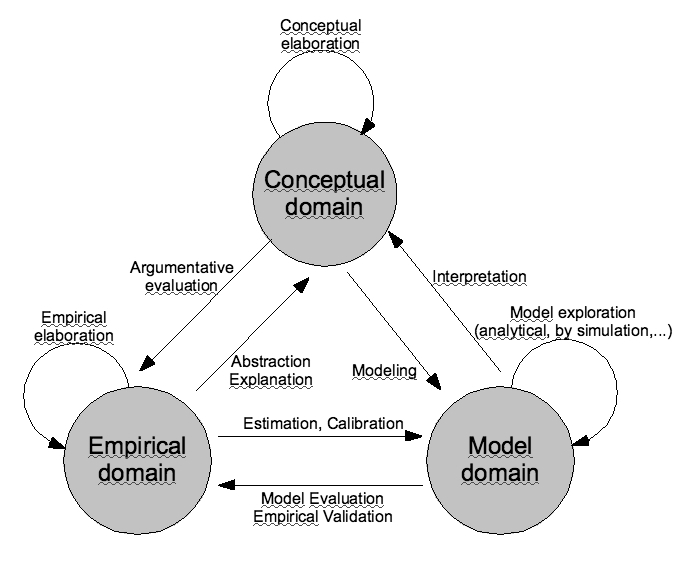
\includegraphics[height=0.55\textheight]{figures/Livet2010_Figure1.jpg}%\hspace{0.1cm}
	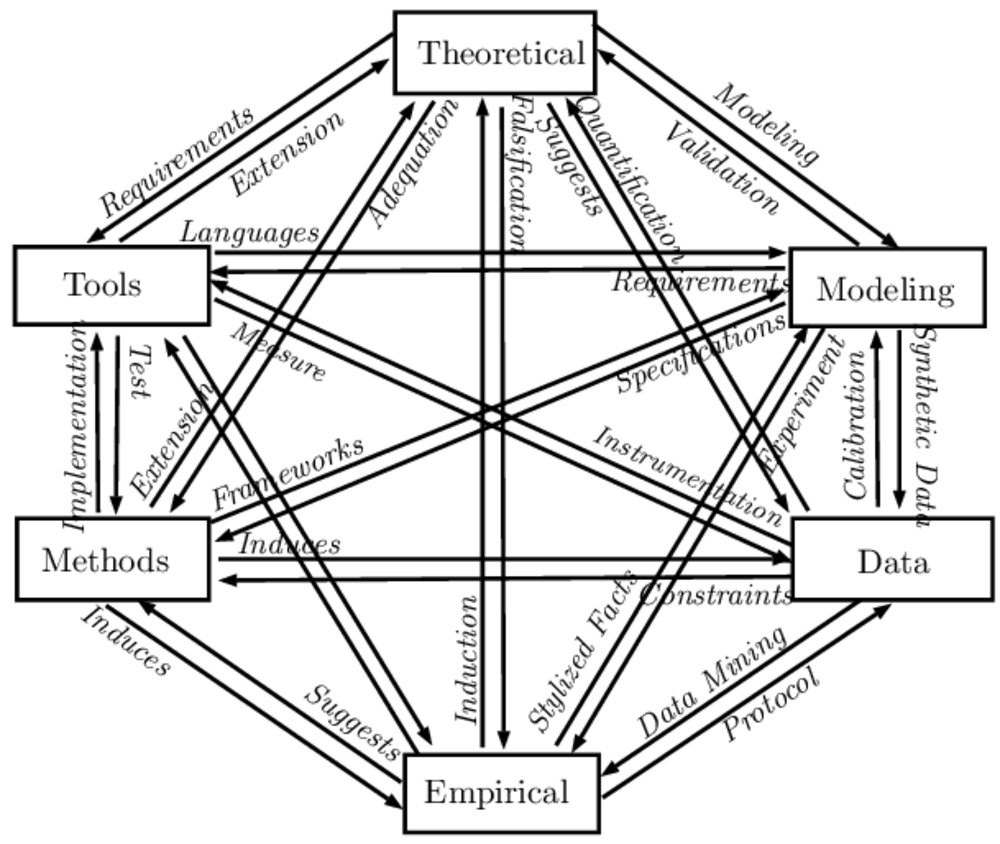
\includegraphics[height=0.55\textheight]{figures/framework.png}
\end{center}

\medskip

\textit{(Left) Knowledge framework for agent-based modelling by \cite{livet2010ontology}; (Right) Refinement with more Knowledge Domains (KDs) by \cite{raimbault2017applied}.}


}

\sframe{KDs in Pumain's Evolutionary Urban Theory}{

% transparent background -> convert
%convert -background white -flatten /home/JRaimbault/ComplexSystems/NetworksTerritories/CityNetwork/Docs/Communications/2017/CSDM2017/figures/openmoleslide.png figures/kd_evolth.png

% second slide with previous work on Denise's theory?

\begin{center}
	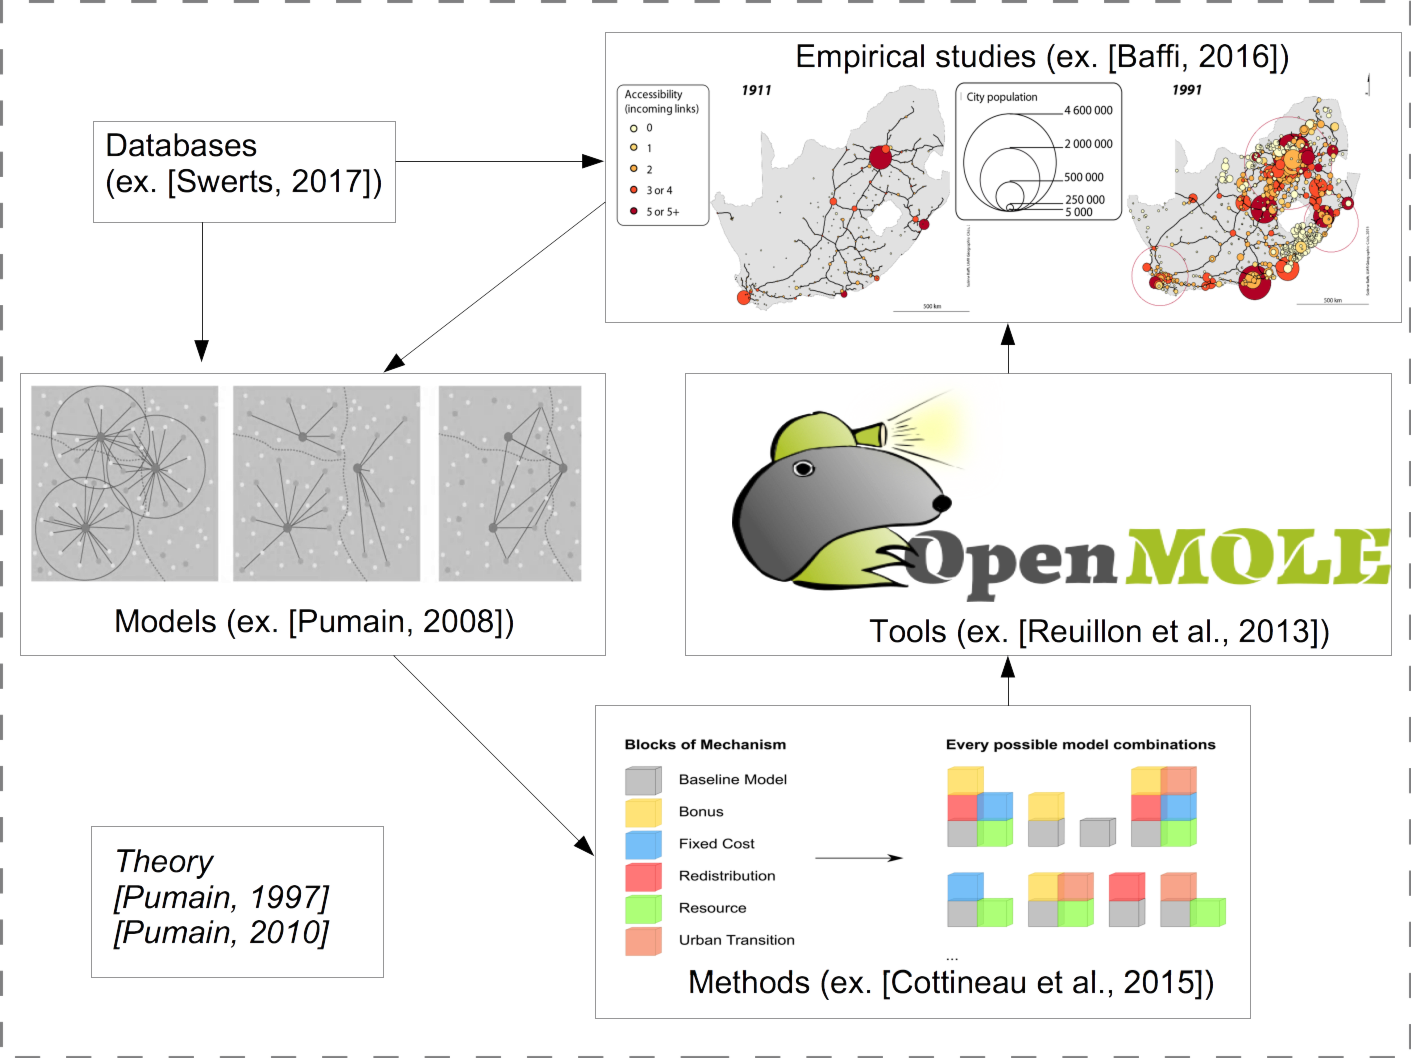
\includegraphics[height=0.8\textheight]{figures/kd_evolth.png}
\end{center}

\footnotesize

\cite{raimbault2017applied}

}


\sframe{Towards a systematic mapping of KDs in TQG}{


% This opens avenues to a systematic mapping of the role of theory in the TQG landscape. However, manual labelling is not achievable for large corpuses. We propose in this contribution to evaluate machine learning methods for an automatic classification of KDs in TQG publications.

\footnotesize

$\rightarrow$ Previous work on Pumain's Evolutionary Urban Theory \cite{pumain2018evolutionary} by \cite{raimbault2017applied} suggested an integration of KDs ; confirmed on larger corpuses (EUT and Zipf's law studies) by \cite{raimbault2025mapping}.

\medskip

$\rightarrow$ More general ongoing epistemological research on TQG: \cite{raimbault2017invisible} (ECTQG 2017),  \cite{raimbault:halshs-02284848} (ECTQG 2019), \cite{raimbault:hal-04257814} (ECTQG 2023).

\medskip

$\rightarrow$ Need to overcome limitations of manual labelling for a systematic mapping of TQG.


\bigskip

\textbf{Research objective:}

\textit{Evaluate machine learning methods for an automatic classification of KDs in TQG publications.}



}


\sframe{Data}{

%  We use the corpus of TheoQuant proceedings (1993-2011, every two years), labelling manually 234 abstracts to obtain training data. Abstracts were first translated into English using the google translate API, as no French domain-specific language model was recently developped for scientific publications.

\begin{itemize}
	\item corpus of TheoQuant proceedings (1993-2011, every two years)
	\item manual labelling of 234 abstracts; multi-class labelling
	\item translation to English using google translate API
	\item four knowledge domains to have enough abstracts in each class : Empirical (125), Theoretical (40), Modelling (56), Methodological (78)


\end{itemize}

% ECTQG single class corpus
%\textbf{Corpus 1: } Pumain's evolutionary urban theory \cite{pumain2018evolutionary}, typical of a fruitful TQG approach (discipline: geography).


}



\sframe{Methods}{

% We then use titles and abstracts concatenated for a multi-binary classification of KDs.
% A baseline model combining tf-idf with a logistic classifier is compared against the SciBERT language model (Beltagy et al., 2019), for a 5-fold cross-validation on the annotated corpus.


\footnotesize

\begin{columns}[T]
        \begin{column}{0.48\textwidth}
            \begin{block}{Baseline: TF-IDF + Logit classifier}
                \begin{itemize}
                    \item \textbf{representation:} sparse vector of term frequencies
                    \item \textbf{focus:} keyword importance
                    \item \textbf{pros:} transparent, fast, low data requirement
                    \item \textbf{cons:} ignores word order and polysemy
                \end{itemize}
            \end{block}
        \end{column}
        
        \begin{column}{0.48\textwidth}
            \begin{block}{Deep Learning: SciBERT \cite{beltagy2019scibert}}
                \begin{itemize}
                    \item \textbf{representation:} pre-trained dense contextual embeddings
                    \item \textbf{focus:} Domain-specific semantics from $1.14M$ papers
                    \item \textbf{pros:} Captures methodological nuance and context
                    \item \textbf{cons:} Computationally expensive, risk of overfitting on small $N$
                \end{itemize}
            \end{block}
        \end{column}
    \end{columns}

    \vspace{0.3cm}


\small \textbf{Training Protocol:} 5-Fold Cross-Validation 

\textbf{Parameters for SciBERT: } 10 epochs, batch size 16, learning rate 2e-5, max seq length 256; local run without GPU %(CPU 10 cores) -> not systematically used by default, no need to specify

%| Threshold Optimization | ZeroR Baseline




}


\begin{frame}{Fine-tuned SciBERT for context-aware classification}
    \begin{itemize}
        \item \textbf{Backbone:} Based on the \textbf{BERT-base} architecture (Bidirectional Encoder Representations from Transformers)
        \begin{itemize}
            \item 12 layers (Transformer blocks)
            \item 768 hidden units and 12 attention heads; \textbf{110M} parameters
            \item links tokens to their context (sentence), in a bidirectional way
        \end{itemize}
        \item \textbf{SciBERT for science: \cite{beltagy2019scibert}}
        \begin{itemize}
            \item \textbf{Vocabulary (SciVocab):} Custom WordPiece vocabulary built from scientific papers (better handling of specific terms like \textit{stochastic} or \textit{model})
            \item \textbf{Pre-training Corpus:} 1.14 million papers from Semantic Scholar
        \end{itemize}
        \item \textbf{Application to TQG (Fine-tuning):}
        \begin{itemize}
            \item Input: Title and Abstract text $\rightarrow$ Output: One of 4 KDs
            \item Training of the classifier via the \textbf{[CLS]} token embedding and a final linear layer for classification
        \end{itemize}
    \end{itemize}
\end{frame}


\sframe{Results: unoptimised classifiers}{

% We obtain a similar performance in terms of F1-score (0.48+-0.05 against 0.46+-0.03 for the baseline), suggesting this classification task is very difficult on abstracts only with no significant improvement for the language model. Hyperparameter tuning for SciBERT seems to slightly improve the performance but still needs further investigation and sensitivity analysis.

\footnotesize

Unoptimised classifiers (probability threshold) do not classify correctly: same performance of random baseline, logit and scibert (F-score $0.48 \pm 0.05$ against $0.46 \pm 0.03$ for the baseline)

\medskip

\textbf{But} models do extract some information: 

\begin{center}
    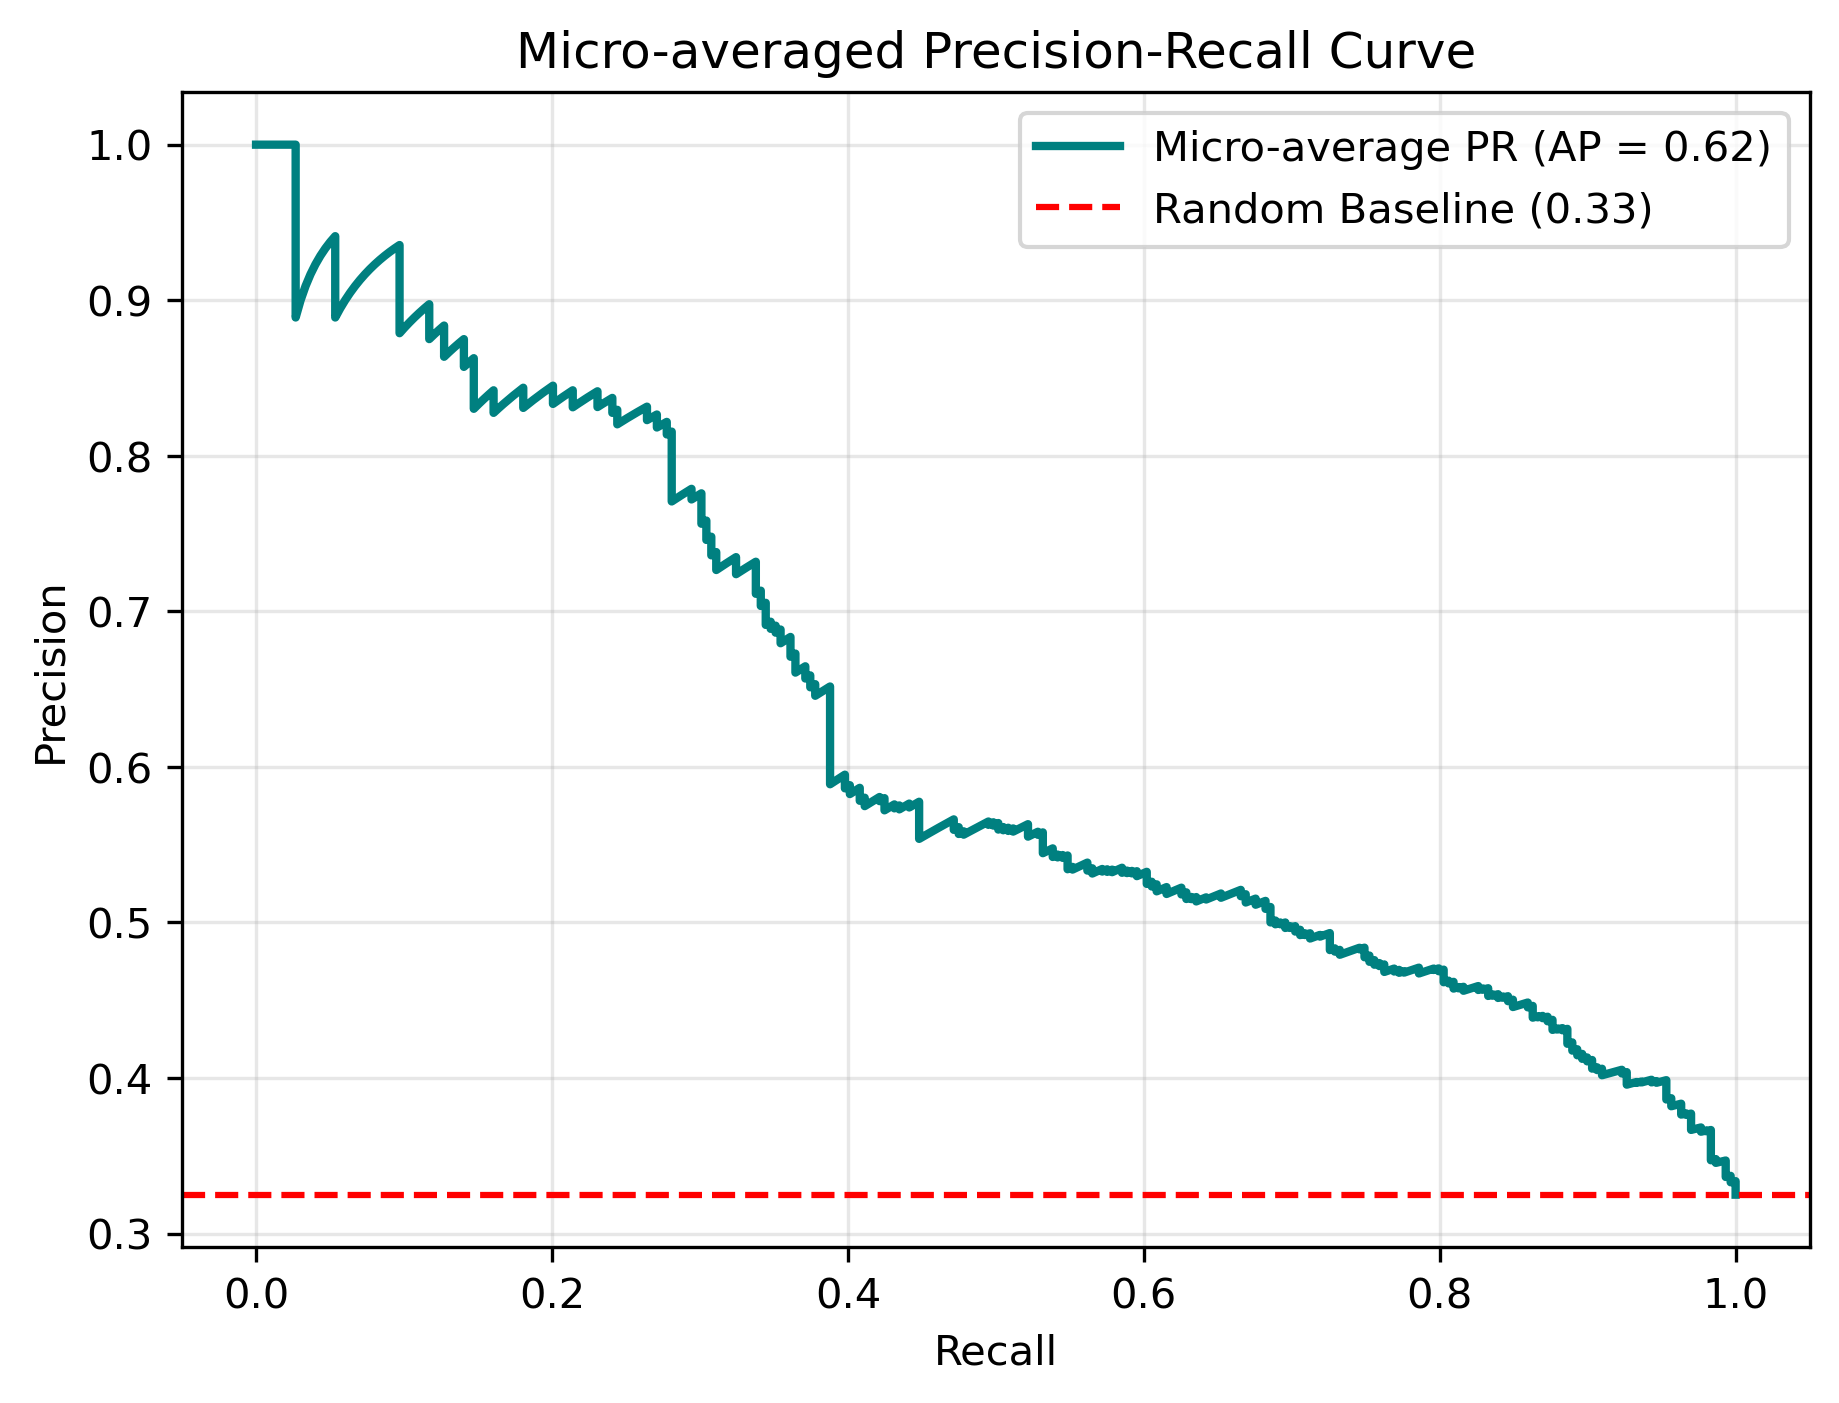
\includegraphics[width=0.5\linewidth]{figures/tfidf-logit-pr-curve_folds5_seed42.png}
\end{center}

\medskip


\textbf{Top terms used by logit: } \textbf{Empirical:} urban, changes; \textbf{Theoretical:} concepts, geography; \textbf{Modelling:} model, simulation; \textbf{Methodological:} variables, method



}

\sframe{Results: optimised thresholds}{

$\rightarrow$ select optimal threshold to classify from predicted probability

\bigskip

\footnotesize

\begin{tabular}{l|ccc}
            \hline
            \textbf{Model} & \textbf{Accuracy} & \textbf{Micro F1} & \textbf{Macro F1} \\
            \hline
            Zero-R (Baseline) & 0.252 ($\pm$0.06) & 0.472 ($\pm$0.06) & 0.175 ($\pm$0.02) \\ 
            TF-IDF + Logit    & 0.274 ($\pm$0.06) & 0.591 ($\pm$0.02) & 0.405 ($\pm$0.08) \\
            \textbf{SciBERT}  & \textbf{0.509 ($\pm$0.05)} & \textbf{0.732 ($\pm$0.02)} & \textbf{0.694 ($\pm$0.04)} \\
            \hline
        \end{tabular}
        
        \medskip




\textit{Accuracy: multi-class exact accuracy; Macro F1: average of F1 scores across all classes; Micro F1: gloobal F1 with sample-level TPs/FPs/FNs}


\bigskip

$\rightarrow$ significant improvment on all indicators

\medskip

$\rightarrow$ with 0.5 accuracy, can be used as a pre-filtering tool but not yet as an automatic classification tool for systematic mapping

}


\sframe{Results: single-class corpus}{


$\rightarrow$ single-class classification, on the Evolutionary Urban Theory corpus ($N=1252$) annotated by \cite{raimbault2025mapping}

\bigskip

\footnotesize

\begin{tabular}{l|ccc}
            \hline
            \textbf{Model} & \textbf{Accuracy} & \textbf{Macro F1} & \textbf{Weighted F1} \\
            \hline
            Zero-R (Baseline) & 0.393 ($\pm$0.03) & 0.141 ($\pm$0.01) & 0.223 ($\pm$0.03) \\ 
            TF-IDF + Logit    & 0.650 ($\pm$0.03) & 0.594 ($\pm$0.03) & 0.650 ($\pm$0.03) \\
            \textbf{SciBERT}  & \textbf{0.798 ($\pm$0.01)} & \textbf{0.743 ($\pm$0.03)} & \textbf{0.796 ($\pm$0.01)} \\
            \hline
        \end{tabular}

\bigskip

$\rightarrow$ again significant improvment on all indicators

\medskip

$\rightarrow$ \textbf{80\% accuracy}, can be used reasonably as a systematic labelling tool


% Ok results last time [11h40~]
% remove this from perspectives
% 	%\item Single-class classification: higher accuracy expected (tfidf-logit gives an accuracy of 0.65 on the EUT corpus by \cite{raimbault2025mapping})


}





\sframe{Discussion}{


%  Our approach opens the way to future applications on larger corpuses, to systematically explore how knowledge is effectively produced in TQG.

% - autres mesures : centralité des differents domaines? (pour influence?)

\footnotesize

\textbf{First results: }
\begin{itemize}
	\item Using a context-aware embedding for scientific texts (SciBERT) for classification \textbf{significantly improves classification}
	\item For multi-class classification, an \textbf{accuracy of 0.5} suggests its use as a \textbf{pre-filtering tool} only; for single-class, an \textbf{accuracy of 0.8} suggests a possible systematic mapping
	\item Promising application of \textbf{deep learning to mapping TQG}
\end{itemize}


\smallskip

\textbf{Perspectives: }

\begin{itemize}
	\item SHAP \cite{mosca2022shap}, hyperparameter optim., GPU training
	\item Test on larger corpuses (e.g. Zipf corpus by \cite{raimbault2025mapping}, $N=858$) and full texts
	\item Application to other tasks: content extraction (model structure \cite{le2026transport}), level of evidence, complexity, \ldots
\end{itemize}

\smallskip

\textbf{Open code and data: } \url{https://github.com/JusteRaimbault/GeoTheoQuantIntegration}

}







%%%%%%%%%%%%%%%%%%%%%
\begin{frame}[allowframebreaks]
\frametitle{References}
\bibliographystyle{apalike}
\bibliography{biblio}
\end{frame}
%%%%%%%%%%%%%%%%%%%%%%%%%%%%




\end{document}

